% Uncomment this line for on-screen presentation
\documentclass[handout, xcolor={dvipsnames}]{beamer}\usepackage{etoolbox}\newtoggle{printable}\togglefalse{printable}

% Uncomment this line for printable slides (disable animations and don't waste ink)
%\documentclass[handout, xcolor={dvipsnames}]{beamer}\usepackage{etoolbox}\newtoggle{printable}\toggletrue{printable}

% Adjust these for the path of the theme and its graphics, relative to this file
%\usepackage{beamerthemeFalmouthGamesAcademy}
\usepackage{../../beamerthemeFalmouthGamesAcademy}
\graphicspath{ {../../} }

% Default language for code listings
\lstset{language=C++}

\begin{document}
\title{Transition to C++ I}   
\subtitle{COMP110: Principles of Computing}

\frame{\titlepage} 

\begin{frame}{Learning outcomes}
	By the end of this session you will
	\begin{itemize}
		\item Understand a thing
		\item Understand another thing
		\item Be convinced that \LaTeX\ makes better-looking slides than PowerPoint
	\end{itemize}
\end{frame}

%\part{Your first C++ program}
\frame{\partpage}

\begin{frame}
	\frametitle{Project setup}
	\begin{itemize}
		\item Open \textbf{Visual Studio 2015} from the Start menu
		\item Click \textbf{New Project}
		\item Choose \textbf{Templates $\to$ Visual~C++ $\to$ Win32 $\to$ Win32~Console~Application}
		\item Choose an appropriate name and location, and click \textbf{OK}
		\item Click \textbf{Finish}
		\item If asked about source control, click \textbf{Cancel}
	\end{itemize}
\end{frame}

\begin{frame}[fragile]
	\frametitle{The code}
	\begin{itemize}
		\item Edit \texttt{$\langle$YourApplicationName$\rangle$.cpp} to match the following:
	\end{itemize}
	\begin{lstlisting}
// YourApplicationName.cpp : Defines the entry point for the console application.

#include "stdafx.h"

int main()
{
    printf("Hello, world!\n");
    return 0;
}
	\end{lstlisting}
\end{frame}

\begin{frame}[fragile]{Running it}
	\begin{itemize}
		\item Click 
\includegraphics[height=2ex]{run_button.png}, or press \textbf{F5} \pause
		\item It worked, but the window disappeared before we could see it! \pause
		\item Solution 1: click \textbf{Debug $\to$ Start~Without~Debugging}, or press \textbf{Ctrl~+~F5}
		\item Solution 2: click in the left margin next to the \lstinline{return 0;} line to set a \textbf{breakpoint} ---
			a red circle should appear. Then click 
\includegraphics[height=2ex]{run_button.png}
	\end{itemize}
\end{frame}

\begin{frame}[fragile]
	\frametitle{Comments}
	\begin{lstlisting}
// ConsoleApplication1.cpp : Defines the entry point for the console application.
	\end{lstlisting}
	\pause
	\begin{itemize}
		\item \lstinline{//} denotes a single-line comment \pause
		\item Equivalent of \lstinline[language=Python]{#} in Python \pause
		\item \textcolor{Gray}{$\hookleftarrow$} denotes a line too long to fit on the slide ---
			in your program this should be a single line \pause
		\item Multi-line comments, delimited by \lstinline{/* */}, are also available
	\end{itemize}
	\begin{lstlisting}
/* This is an example of a multi-line comment
   More comment text
   Even more comment text */
	\end{lstlisting}
\end{frame}

\begin{frame}[fragile]
	\frametitle{The \#include directive}
	\begin{lstlisting}
#include "stdafx.h"
	\end{lstlisting}
	\pause
	\begin{itemize}
		\item \lstinline{#include} imports definitions from a \textbf{header file} \pause
		\item Similar to \lstinline[language=Python]{import} in Python \pause
		\item \lstinline{#include "..."} (quotes) is used for headers in the current project \pause
		\item \lstinline{#include <...>} (angle brackets) is used for external libraries \pause
		\item \texttt{stdafx.h} is the \textbf{precompiled header} file --- for faster compilation, external library headers should be included here rather than in the main \texttt{.cpp} file
	\end{itemize}
\end{frame}

\begin{frame}[fragile]
	\frametitle{Entry point}
	\begin{lstlisting}
int main()
	\end{lstlisting}
	\pause
	\begin{itemize}
		\item \textbf{All code} must be inside a \textbf{function} \pause
		\item The \textbf{entry point} of an application is (almost) always named \lstinline{main} \pause
		\begin{itemize}
			\item Some types of Windows GUI application use a different name for the entry point \pause
			\item A game engine (e.g.\ Unreal) takes care of the entry point for you \pause
		\end{itemize}
		\item \lstinline{int} means the function \textbf{returns} a value of integer type \pause
		\item \lstinline{()} means the function takes \textbf{no parameters}
	\end{itemize}
\end{frame}

\begin{frame}[fragile]
	\frametitle{Blocks and semicolons}
	\begin{lstlisting}
{
    ...;
    ...;
}
	\end{lstlisting}
	\pause
	\begin{itemize}
		\item Curly braces are used to denote \textbf{blocks} \pause
		\item All statements in C++ end with a semicolon \lstinline{;} \pause
		\item Unlike Python, C++ ignores whitespace (indentation and usually line breaks) \pause
		\item ... but whitespace is important for readability, so use it anyway
	\end{itemize}
\end{frame}

\begin{frame}[fragile]
	\frametitle{Writing to the console}
	\begin{lstlisting}
    printf("Hello, world!\n");
	\end{lstlisting}
	\pause
	\begin{itemize}
		\item Equivalent of Python's \lstinline[language=Python]{print} statement \pause
		\item \lstinline{printf} is a function, part of the \textbf{standard library} \pause
		\item In Unreal, can use \lstinline{UE_LOG} for the same purpose \pause
		\item \lstinline{"\n"} is the \textbf{new line character} \pause
		\item Most online tutorials will recommend using \lstinline{std::cout} to write to console,
			but \lstinline{printf} is easier for now
	\end{itemize}
\end{frame}

\begin{frame}[fragile]{Formatted printing}
	\pause
	\begin{itemize}
		\item The string passed to \lstinline{printf} can include \textbf{placeholders} \pause
		\item Pass further arguments to \lstinline{printf}, one for each placeholder \pause
	\end{itemize}
	\begin{lstlisting}
printf("%d plus %d equals %d\n", 3, 4, 3+4);
	\end{lstlisting}
	\begin{itemize}
		\item Placeholder \textbf{must} match the type of the argument \pause
		\item \lstinline{"%d"} or \lstinline{"%i"}: integer \pause
		\item \lstinline{"%f"}: floating point \pause
		\item \lstinline{"%s"}: string
	\end{itemize}
\end{frame}

\begin{frame}[fragile]
	\frametitle{Exit code}
	\begin{lstlisting}
    return 0;
	\end{lstlisting}
	\pause
	\begin{itemize}
		\item Returning 0 from \lstinline{main} tells the OS that the program completed successfully \pause
		\item Mainly useful for writing tools to be used in DOS/Windows batch scripts or Linux shell scripts ---
			for our purposes, \lstinline{main} will almost always return 0
	\end{itemize}
\end{frame}


%\part{Variables and types}
\frame{\partpage}

\begin{frame}[fragile]{Variables}
	\begin{columns}[onlytextwidth]
		\begin{column}{0.45\textwidth}
			In Python, variables exist the moment they are assigned to:
			\begin{lstlisting}[language=Python]
a = 10
b = 20
			\end{lstlisting}
			\pause
			Variables can hold values of any type:
			\begin{lstlisting}[language=Python]
a = 10
a = 3.14159
a = "Hello"
			\end{lstlisting}
		\end{column}
		\pause
		\begin{column}{0.45\textwidth}
			In C++, variables must be \textbf{declared} before use, and must be given a \textbf{type}:
			\begin{lstlisting}
int a = 10;
int b = 20;
			\end{lstlisting}
			\pause
			Variables can only hold values of the correct type:
			\begin{lstlisting}
int a = 10;
a = 17;      // OK
a = "Hello"; // Error
			\end{lstlisting}
		\end{column}
	\end{columns}
\end{frame}

\begin{frame}[fragile]{Integers}
	\begin{itemize}
		\item \lstinline{int} is the basic data type for integers (whole numbers)
	\end{itemize}
	\begin{lstlisting}
int a = 42;
int b = -74965;
int c = 0;
int d = 0x19FD; // Hexadecimal
	\end{lstlisting}
	\pause
	\begin{itemize}
		\item On Windows (32 and 64 bit), \lstinline{int} can store numbers from $-2^{31}$ to $2^{31}-1 \approx \pm 2$ billion \pause
		\item \lstinline{unsigned int} stores \textbf{nonnegative} integers, from 0 to $2^{32} \approx 4$ billion \pause
		\item Other integer types exist, for example \lstinline{long long} is a 64 bit integer
	\end{itemize}
\end{frame}

\begin{frame}[fragile]{Floating point numbers}
	\begin{itemize}
		\item \lstinline{float} and \lstinline{double} can store floating point numbers (numbers with a fractional part)
	\end{itemize}
	\begin{lstlisting}
double a = 3.14159;
double b = -42;
double c = 3.0e8; // Scientific notation
float d = 123.456f; // Note the 'f' suffix for float
	\end{lstlisting}
	\pause
	\begin{itemize}
		\item \lstinline{float} uses less space, and can be slightly faster, but is less precise \pause
		\item Generally \lstinline{double} is the better choice
	\end{itemize}
\end{frame}

\begin{frame}[fragile]{Characters}
	\begin{itemize}
		\item \lstinline{char} stores a single ASCII character
	\end{itemize}
	\begin{lstlisting}
char foo = 'Q';
char bar = '7';
char baz = '@';
char space = ' ';
char newLine = '\n'; // Escape sequence
	\end{lstlisting}
	\pause
	\begin{itemize}
		\item \lstinline{char} can also be thought of as an 8-bit integer, i.e. an integer between $-128$ and $127$ ---
			C++ makes no distinction between ASCII characters and their numerical codes
	\end{itemize}
\end{frame}

\begin{frame}[fragile]{Booleans}
	\begin{itemize}
		\item \lstinline{bool} stores a boolean (true or false) value
	\end{itemize}
	\begin{lstlisting}
bool isAlive = true;
bool isDead = false;
	\end{lstlisting}
\end{frame}

\begin{frame}[fragile]{Vectors}
	\begin{itemize}
		\item \textbf{Vectors} are the C++ equivalent of lists in Python
		\pause
		\item Add \lstinline{#include <vector>} to \texttt{stdafx.h}
		\pause
		\item \lstinline{std::vector<T>} is a vector with elements of type \lstinline{T}
	\end{itemize}
	\pause
	\begin{lstlisting}
std::vector<int> numbers = { 1, 4, 9, 16 };
numbers.push_back(25);
	\end{lstlisting}
\end{frame}

\begin{frame}[fragile]{Strings}
	\begin{itemize}
		\item C++ has two main data types for strings:
		\begin{itemize}
			\item \lstinline{char*} or \lstinline{char[]}: low-level array of ASCII characters (more on arrays next week)
			\item \lstinline{std::string}: high-level string class
		\end{itemize}
		\pause
		\item Use \lstinline{std::string} unless you have a compelling reason not to
		\pause
		\item Add \lstinline{#include <string>} to \texttt{stdafx.h}
	\end{itemize}
	\pause
	\begin{lstlisting}
std::string name = "Ed";
std::string message = "Hello " + name + "!";
std::cout << message << std::endl;
	\end{lstlisting}
\end{frame}

\begin{frame}[fragile]{Enumerations}
	\begin{itemize}
		\item An \textbf{enumeration} is a set of named values
	\end{itemize}
	\pause
	\begin{lstlisting}
enum Direction { dirUp, dirRight, dirDown, dirLeft };

Direction playerDirection = dirUp;
	\end{lstlisting}
	\pause
	\begin{itemize}
		\item This is equivalent to using an \lstinline{int} with 0=up, 1=right etc, but is more readable
	\end{itemize}
\end{frame}

\begin{frame}[fragile]{Constants}
	\begin{itemize}
		\item The \lstinline{const} keyword can be used to define a ``variable'' whose value cannot change, i.e.\ read only
	\end{itemize}
	\pause
	\begin{lstlisting}
const int x = 7;
std::cout << x << std::endl; // OK
x = 12; // Error
	\end{lstlisting}
\end{frame}

\begin{frame}[fragile]{Declaring variables}
	\begin{itemize}
		\item A variable declaration must specify a \textbf{type}, and one or more \textbf{variable names}:
	\end{itemize}
	\begin{lstlisting}
int i, j, k;
bool isDead;
std::string playerName;
	\end{lstlisting}
	\pause
	\begin{itemize}
		\item A variable declaration can optionally specify an \textbf{initial value}:
	\end{itemize}
	\begin{lstlisting}
int i = 0, j = 1, k = 2;
bool isDead = false;
std::string playerName = "Ed";
	\end{lstlisting}
\end{frame}

\begin{frame}[fragile]{Initial values}
	\begin{itemize}
		\item If the initial value is omitted, what happens depends on the type: \pause
		\item Basic data types (\lstinline{int, double, bool, char} etc): the value is undefined --- whatever data happened
		to be in that memory location already \pause
		\begin{itemize}
			\item Your code should \textbf{never} read an uninitialised variable --- doing so is \textbf{always} a bug \pause
		\end{itemize}
		\item Object types (\lstinline{std::vector, std::string} etc): depends on the type (consult the documentation) \pause
		\begin{itemize}
			\item \lstinline{std::vector} and \lstinline{std::string} are both initialised to empty
		\end{itemize}
	\end{itemize}
\end{frame}

\begin{frame}[fragile]{Scope}
	\begin{itemize}
		\item The \textbf{scope} of a variable is the region of the program where it exists \pause
		\item Generally the scope of a variable begins when it is declared,
		and ends when the block in which it is declared ends \pause
	\end{itemize}
	\begin{lstlisting}
int x = 7;
if (x > 5)
{
    int y = x * 2;
    std::cout << x << std::endl; // OK
    std::cout << y << std::endl; // OK
}
std::cout << x << std::endl; // OK
std::cout << y << std::endl; // Error
	\end{lstlisting}
\end{frame}


\part{Control structures}
\frame{\partpage}

\begin{frame}[fragile]{If statement}
	\begin{lstlisting}
if (x > 0)
{
    std::cout << "x is positive" << std::endl;
}
else if (x < 0)
{
    std::cout << "x is negative" << std::endl;
}
else
{
    std::cout << "x is neither positive nor negative" << std::endl;
}
	\end{lstlisting}
    \pause
    \begin{itemize}
        \item Condition is always in parentheses \lstinline{( )}
    \end{itemize}
\end{frame}

\begin{frame}[fragile]{Conditions}
    \begin{itemize}
        \item Numerical comparison operators work just like Python:
        \lstinline{==  !=  <  >  <=  >=}
        \item Boolean logic operators look a little different
    \end{itemize}
    Python uses \lstinline[language=Python]{and, or, not}
    \begin{lstlisting}[language=Python]
if not (x < 0 or x > 100) and not (y < 0 or y > 100):
    print "Point is in rectangle"
    \end{lstlisting}
    C++ uses \lstinline{&&, ||, !}
    \begin{lstlisting}[language=Python]
if (!(x < 0 || x > 100) && !(y < 0 || y > 100))
{
    std::cout << "Point is in rectangle" << std::endl;
}
    \end{lstlisting}
\end{frame}

\begin{frame}[fragile]{Single-statement blocks}
    \begin{itemize}
        \item In many cases, if a block contains only a single statement then the curly braces can be omitted
    \end{itemize}
    \begin{lstlisting}
if (x > 0)
    std::cout << "x is positive" << std::endl;
else if (x < 0)
    std::cout << "x is negative" << std::endl;
else
    std::cout << "x is neither positive nor negative" << std::endl;
    \end{lstlisting}
    \begin{itemize}
        \item Careful though! This can lead to obscure bugs
    \end{itemize}
    \begin{lstlisting}
// This code is wrong!
if (z == 0)
    x = 0; y = 0;
    \end{lstlisting}
\end{frame}

\begin{frame}[fragile]{Switch statement}
	\begin{lstlisting}
switch (x)
{
case 0:
    std::cout << "zero" << std::endl;
    break;
case 1:
    std::cout << "one" << std::endl;
    break;
case 2:
    std::cout << "two" << std::endl;
    break;
default:
    std::cout << "something else" << std::endl;
    break;
}
	\end{lstlisting}
\end{frame}

\begin{frame}[fragile]{While loop}
	\begin{lstlisting}
while (x > 0)
{
    std::cout << x << std::endl;
    x--;
}
	\end{lstlisting}
\end{frame}

\begin{frame}[fragile]{Do-while loop}
	\begin{lstlisting}
do
{
    std::cout << x << std::endl;
    x--;
} while (x > 0);
	\end{lstlisting}
	\pause
	\begin{itemize}
		\item \lstinline{while} loop checks the condition \textbf{before} executing the loop body \pause
		\item \lstinline{do-while} loop checks the condition \textbf{after} executing the loop body \pause
		\item e.g. if \lstinline{x == 0} to begin with, the \lstinline{while} body does not execute, the \lstinline{do-while} body executes once
	\end{itemize}
\end{frame}

\begin{frame}[fragile]{For-each loop}
	\begin{lstlisting}
std::vector<int> numbers { 1, 3, 5, 7, 9 };

for each (int x in numbers)
{
    std::cout << x << std::endl;
}
	\end{lstlisting}
    \pause
	\begin{itemize}
		\item This works like the \lstinline{for} loop in Python
		\item Used for iterating over data structures
	\end{itemize}
\end{frame}

\begin{frame}[fragile]{For loop}
	\begin{lstlisting}
for (int i = 0; i < 10; i++)
{
    std::cout << i << std::endl;
}
	\end{lstlisting}
	\pause
    \begin{itemize}
        \item The \lstinline{for} loop has three parts: \pause
        \item The \textbf{initialiser} \lstinline{int i = 0}
        \begin{itemize}
            \item This is executed at the start of the loop
        \end{itemize} \pause
        \item The \textbf{condition} \lstinline{i < 10}
        \begin{itemize}
            \item The loop executes while this evaluates to \lstinline{true}
        \end{itemize} \pause
        \item The \textbf{loop statement} \lstinline{i++}
        \begin{itemize}
            \item This is executed at the end of each iteration of the loop
        \end{itemize}
    \end{itemize}
\end{frame}

\begin{frame}[fragile]{For loops and while loops}
	\begin{lstlisting}
for (int i = 0; i < 10; i++)
{
    std::cout << i << std::endl;
}
	\end{lstlisting}
    \begin{itemize}
        \item Any \lstinline{for} loop can easily be rewritten as a \lstinline{while} loop
    \end{itemize}
    \pause
	\begin{lstlisting}
int i = 0;
while (i < 10)
{
    std::cout << i << std::endl;
    i++;
}
	\end{lstlisting}
\end{frame}

\begin{frame}[fragile]{For loops in C++ and Python}
	\begin{lstlisting}
for (int i = 0; i < 10; i++)
{
    std::cout << i << std::endl;
}
	\end{lstlisting}
    \begin{itemize}
        \item In Python, this would be written as a for-each loop, first using the \lstinline[language=Python]{range} function
        to construct the list of numbers $0, 1, 2, \dots, 9$:
    \end{itemize}
	\begin{lstlisting}[language=Python]
for i in range(10):
    print i
	\end{lstlisting}
\end{frame}



% -------------------------------------------------------

%\part{The compiler}
%\frame{\partpage}
%
%\begin{frame}
%	\frametitle{The build process}
%	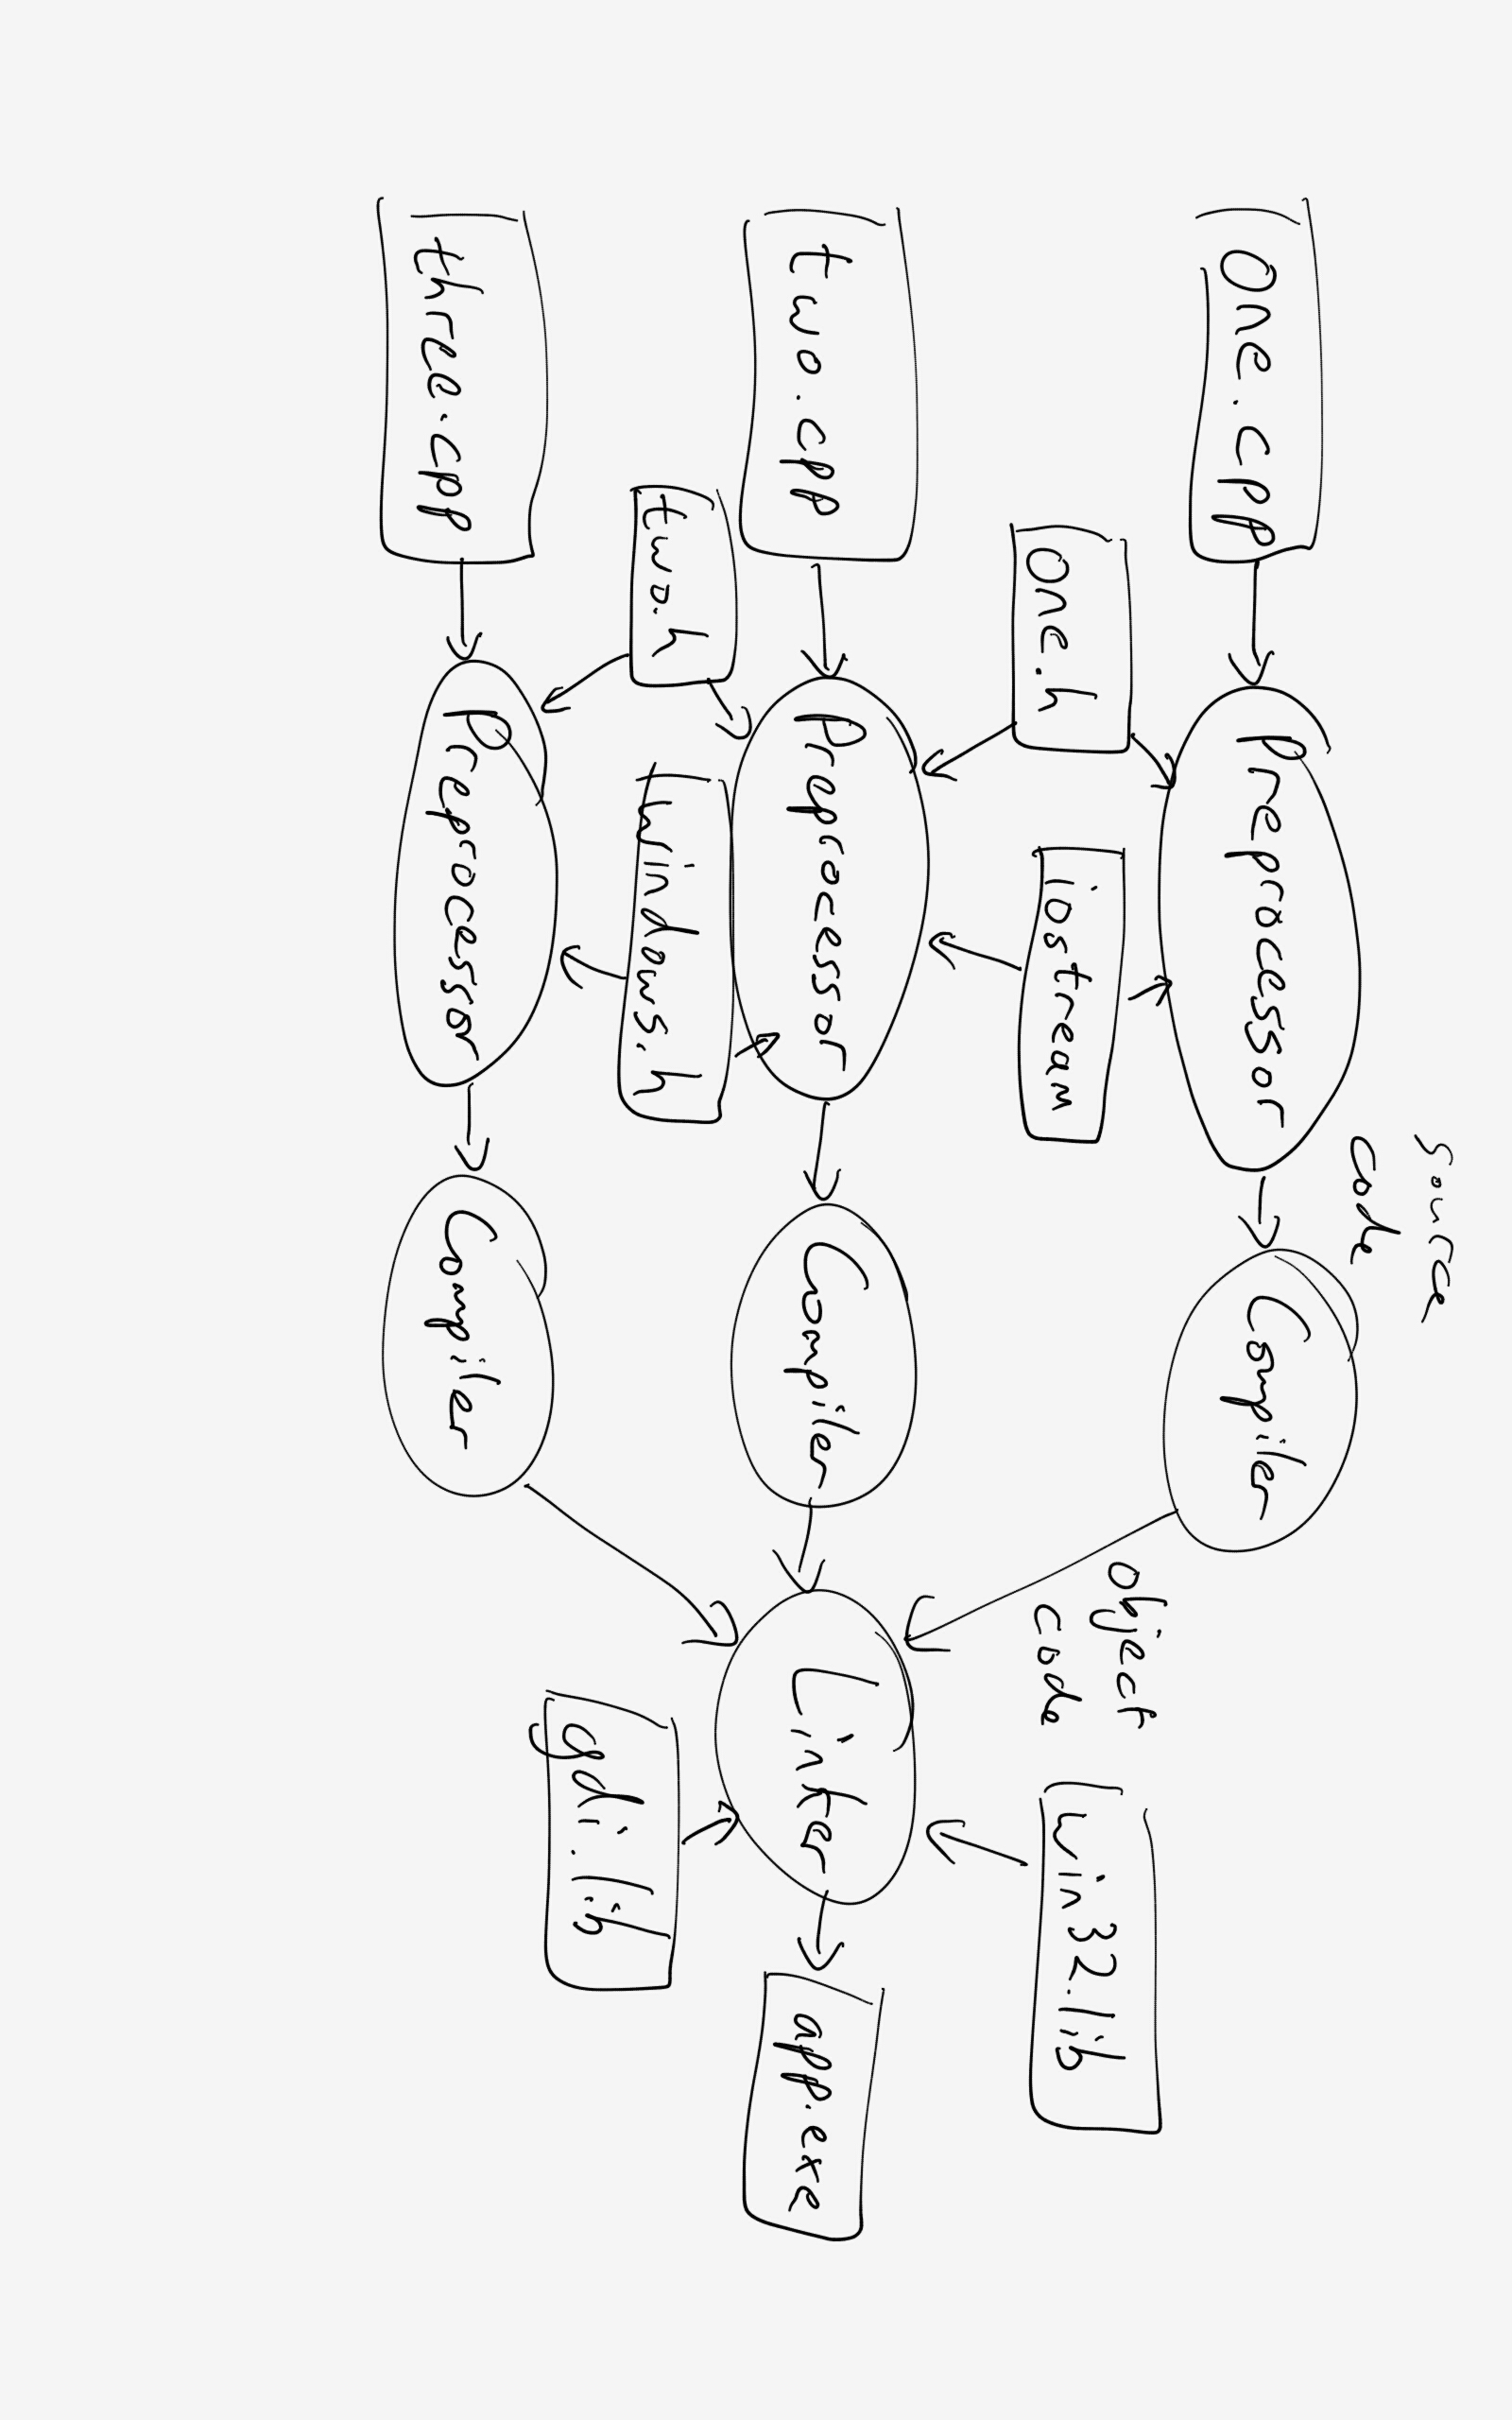
\includegraphics[height=\textwidth,angle=90]{compiler_sketch}
%\end{frame}

\end{document}
